The rock block generating algorithm is based on a subdivision approach: each discontinuity is introduced sequentially and if it intersects the parent block, the parent block is subdivided into two child blocks. This process is repeated until all discontinuities have been processed and is repeated for each block. Figure \ref{fig:SlicingIllustration} shows a simple schematic of this process. The original serial algorithm is implemented in C++ using data structures to represent the blocks and discontinuities. \par 

\begin{figure}[h]
  \centering
  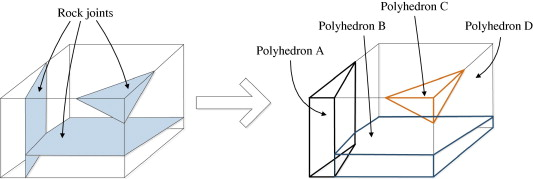
\includegraphics[width=0.4\textwidth]{SlicingIllustration}
  \caption{Polyhedron generation schematic \cite{slicing}}
  \label{fig:SlicingIllustration}
\end{figure}

This algorithm is refactored and modified in Scala to run in parallel on Spark using a functional approach. The following sections give a description of how the different stages of the rock generation process are implemented from a high level. \ref{Details} gives more detail on the actual code generated to do this.  Within Scala, the blocks are case classes that keep a list of faces that define the block as well as the location of its center in global coordinates. The faces are are objects that store the face's normal vector, a distance from the block's origin, as well as the friction angle and cohesion along the face. The discontinuities, or joints, are also case classes. The class contains the normal vector to the plane that defines the joint, its distance from the joint's local origin and the global coordinates that define that origin. Additionally, it stores the dip angle, dip direction (shown in Figure \ref{fig:DipFig}), friction angle and cohesion along the joint face. In the case of non-persistent joints, it also stores a list of inequalities that describe the shape of the joint. 

\begin {figure}[h]
  \centering
  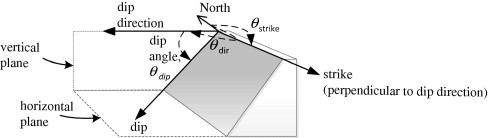
\includegraphics[width=0.4\textwidth]{DipFig}
  \caption{Definition of strike, dip and dip direction \cite{slicing}} 
  \label{fig:DipFig}           
\end{figure}

Using this data structure, it is possible to completely describe the volume defining a polyhedral block, negating the need to story any information on the edges and vertics which can be calculated if necessary. The volume defining a block bounded by \textit{N} planes can be described completely by the following inequality:

\begin{equation}
a_ix + b_iy + c_iz \leq d_i, i = 1,...,N 
\end{equation}

The coefficients $(a_i, b_i, c_i)$ represent the normal vector to the $i^{th}$ plane bounding the block and $d_i$ is the distance of that plane from some local origin. \par
 
In order to subdivide blocks, it is necessary to determine whether block is intersected

\subsection{Input Processing}
